% Synthetic placeholder figure generated from experiment/sec-5-rq1-native-code/data/microbench.csv
\begin{figure*}[t]
  \centering
  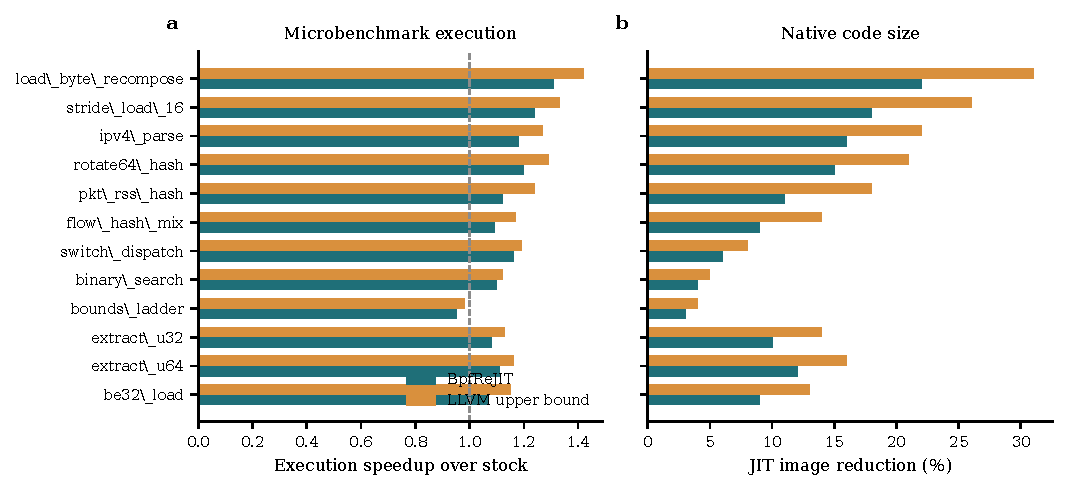
\includegraphics[width=\linewidth]{figures-next/rq1-micro-overview.pdf}
  \caption{Supported-family microbenchmarks. Across these synthetic placeholder results, \tool achieves a geometric-mean 1.13x speedup over the stock kernel JIT together with a median 10.5\% JIT-image reduction. LLVM remains a stronger upper bound, but \tool closes most of the visible gap on wide-memory and rotate-heavy programs. \note{rq-1-exp-1}}
  \label{fig:rq1-micro-overview}
\end{figure*}
